
\chapter{Exact Models}
The previous sections illustrated some heuristic methods. The main property of those methods is their speed, but they provide approximate solutions. In contrast, to obtain the best possible solution, we must use exact methods that optimize a mathematical model of the problem and find the optimal solution.

This section introduces methods that solve a MIP problem to optimality using the basic CPLEX \cite{Cplex:TSP} MIP solver. The MIP problem model used is described in the introduction section \ref{chap:DFJ}.

The main challenge was adding the sub-tour elimination constraints (SEC) \ref{eq:eq3}. The initial approach was to define and build a model without these constraints and directly use the CPLEX solver on it. Obviously, this approach yields an incorrect solution composed of various separated components instead of a unique path that visits all points.

To address this problem, the first method that we propose is Benders' Loop, which iteratively adds the SEC and solves the problem until the optimal solution without subtours is found. The second method uses a CPLEX callback function that is called every time a new solution is found. This allows us to reject solutions with subtours by adding the corresponding SECs or to accept the solution if it has only one component.
We will also cover some other methods that can speed up the process, such as Posting heuristic solutions, MIP start and User-cut callbacks.

\section{Benders' Loop method}
The Dantzig-Fulkerson-Johnson (DFJ) \ref{chap:DFJ} model incorporates subtour elimination constraints to the problem, but the number of such constraints is exponential.

The first method we introduce to address this issue is known as "Benders' Loop". This method is based on the idea that the majority of potential subtours consist of very unfavorable edge combinations, which correspond to parts of the solution space that the MIP solver would quickly discard while minimizing the solution cost. Therefore, the method focuses only on the subtours selected by the solver, prohibiting their selection.

Benders' implementation iteratively solves the DFJ model. It begins with the degree constraints and solves the problem using CPLEX's MIP solver. Upon finding a solution, it checks for the presence of subtours. If subtours are detected, the method adds subtour elimination constraints (SECs) for each subtour and resolves the modified model until a solution is found or the time limit is reached. Specifically, if the solution contains \( m \) subtours and \( S_k \) is a subtour, the Loop method adds the following constraints:

\[
\sum_{e \in E(S_k)} x_e \leq |S_k| - 1 \quad \text{for} \; k = 1, \ldots, m
\]

The pseudo-code of Benders’ loop method is shown in Algorithm~\ref{alg:Bender}.

\begin{algorithm}[H]
    \caption{Benders implementation of the DFJ model}
    \label{alg:Bender}
    \begin{spacing}{1.2} % Adjust this value to change line spacing
        \KwIn{TSP instance}
        \KwOut{A valid tour (CPLEX solution)}
        \BlankLine
        model \leftarrow $naive\_model$\;
        solution \leftarrow $solve$ model\;

        \While{solution \textbf{has} $subtours$}
        {
            \ForEach{subtour \textbf{in} solution}
            {
                sec\_constraints \leftarrow generate SECs constraints of subtour\;
                \textbf{add} sec\_constraints \textbf{to} model\;
            }
            solution \leftarrow $solve$ model
        }
        \BlankLine
    \end{spacing}
\end{algorithm}

This procedure avoids generating an exponential number of constraints. However, the major drawback is the need to rebuild and reoptimize the model from scratch at each iteration.

\subsection{Patching Heuristic for Benders: Gluing}
The Bender's Loop method, in every iteration, only creates new SECs and then discards all previous work to start again from scratch. Instead, it would be beneficial to save as much progress as possible to make the method more efficient. A possible solution is to attempt to fix the solution provided by CPLEX by gluing together the subtours, resulting in a single comprehensive path.

The output of this technique will not have any guaranteed optimality, but it could still be valuable. In case the method is stopped before completion, we would have a feasible solution. Additionally, it can provide a good upper bound, as we know that the optimal solution will have a cost better than or equal to the glued solution. Moreover, it offers a good starting point for the next iteration, as the glued solution can be provided to CPLEX as a MIP start.

The action of gluing together two subtours is made by choosing the best couple of edges of different components that generate the lowest difference of cost when swapped (as shown in Figure \ref{fig:patch_img}). This operation is repeated until there is only one component.

\begin{figure}
    \centering
    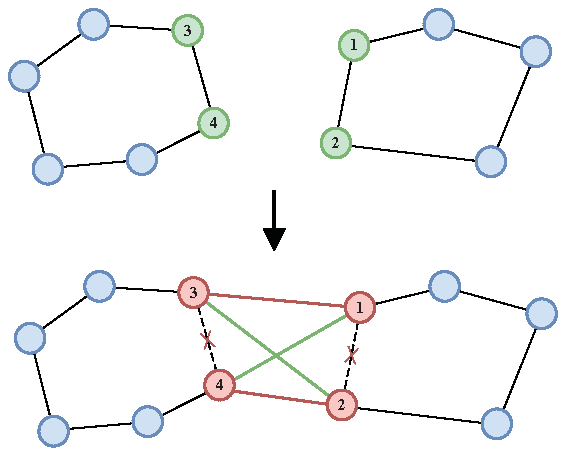
\includegraphics[width=0.8\linewidth]{Immagini/patch.pdf}
    \caption{Gluing of two components.}
    \label{fig:patch_img}
\end{figure}

\newpage

The pseudo-code of the gluing operation is shown in Algorithm~\ref{alg:gluing}. It takes as input the multi-component solution in a particular format:
\begin{itemize}[noitemsep]
    \item \texttt{ncomps}: number of components
    \item \texttt{comp}: array with ids of components for each node
    \item \texttt{succ}: array with successive node of each node
    \item \texttt{cost}: cost of the current solution
\end{itemize}

\begin{algorithm}[H]
    \caption{Gluing}
    \label{alg:gluing}
    \begin{spacing}{1.3} % Adjust this value to change line spacing
        \KwIn{ncomps, comp, succ, cost}
        \KwOut{The glued solution}
        \BlankLine
        \While{\textit{ncomp > 1}}
        {
            edge1, edge2, costDifference \leftarrow \textbf{find} \ \textit{best (with minimum cost difference) 2 edges to} \textbf{swap} \textit{such that they are from different components}\;
            
            \BlankLine
            \textbf{swap} \textit{succ[edge1.first]} \textbf{with} \textit{succ[edge2.first]}\;
            \textbf{update} value of \textit{comp} to values in range \textit{[1, ncomp-1]}\;

            \BlankLine
            cost \leftarrow \textit{cost + costDifference}\;
            ncomp \leftarrow \textit{ncomp - 1}\;
        }
        \BlankLine
    \end{spacing}
\end{algorithm}

\section{Branch and Cut in CPLEX with candidate callback}

An alternative method to incorporate SEC constraints is through the branch-and-cut technique, specifically utilizing CPLEX to address the problem. 

At the root node, CPLEX’s branch-and-cut algorithm performs several preprocessing steps. For each node in the branching tree (Figure \ref{fig:bec_img}), it employs multiple cut separation families, such as Gomory, Clique, and 0-1/2 cuts. Following the calculation of the relaxation, primal heuristics are applied to identify increasingly optimal incumbent solutions. These heuristics take the fractional solution as input, convert it into an integer solution, and if the resulting cost is lower than the current incumbent solution, the incumbent is updated. This integer solution may still contain subtours. 


\begin{figure}[H]
    \centering
    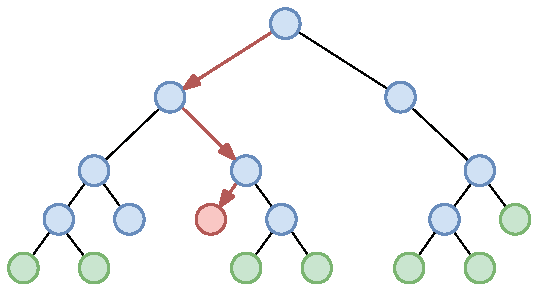
\includegraphics[width=0.9\linewidth]{Immagini/bec.pdf}
    \caption{Branch \& Cut tree visualization.}
    \label{fig:bec_img}
\end{figure}

Between the heuristic application and the incumbent update, it is possible to instruct CPLEX to invoke a custom callback function. Exploiting this CPLEX feature we can inspect the solution and act based on its properties. If it has sub-tours the function adds the SECs and discards the solution, while if it has only one component the function accepts it.

This method let use fully use the potential of CPLEX without needing to restart the optimization multiple times.

The pseudo-code of the candidate callback is shown in Algorithm~\ref{alg:cand_callback}.\\

\begin{algorithm}[H]
    \caption{Candidate callback}
    \label{alg:cand_callback}
    \begin{spacing}{1.2} % Adjust this value to change line spacing
        \KwIn{Candidate solution}
        \BlankLine
        \If{solution \textbf{has} subtours}
        {
            \ForEach{subtour \textbf{in} solution}
            {
                sec\_constraints $\leftarrow$ generate SECs constraints of subtour\;
                \textbf{add} sec\_constraints to model\;
                \textbf{discard} solution\;
            }
        }
        \Else
        {
            \textbf{accept} solution\;
        }
        \BlankLine
    \end{spacing}
\end{algorithm}

\newpage

\subsection{Posting Heuristic solutions}
The incumbent callback allows for the implementation of custom heuristics to help CPLEX quickly identify an improved solution.

Starting with the integer solution provided by CPLEX in this callback, the gluing algorithm from the Bender's loop method can be applied, followed by a 2-opt optimization.

The improved solution can then be \textit{posted} in the CPLEX environment, making it available for evaluation. CPLEX will assess this solution and determine whether to adopt or discard it.

\subsection{MIP start}
In addition to the aforementioned techniques, it is also possible to provide a starting solution to CPLEX, known as a MIP start, which prevents the creation of poor random solutions at the beginning of the Branch-and-Cut (B\&C) method. By doing so, the CPLEX solver can begin its optimization process with a reasonably good feasible solution, working to improve it towards optimality rather than starting from a random solution, which may be much more challenging to optimize.

To generate the MIP start solution, any of the previously discussed heuristic or metaeuristic methods can be employed. In our case, we decided to use a simple nearest neighbor heuristic starting from a random node, combined with a 2-opt optimization: a suitable balance between a fast and robust approach.

\section{SECs for Fractional solutions: user-cut callback}
In this section, we describe an advanced use of CPLEX’s callback functionality. At each node of the branching tree, CPLEX allows the invocation of a user-cut callback, a custom function applied to the relaxed solution of the problem. The relaxed solution does not account for the integer constraints of the variables. This feature facilitates the creation of custom cuts for the relaxed problem using callbacks. However, in the context of the TSP, the solution must be integer. Consequently, the methods used in previous sections to count the number of components or to merge them are not applicable.

To address this, functions from the Concorde library are utilized \cite{conc}. For example, the function \texttt{CCcut\_connect\_components} counts the components in a fractional solution, and \texttt{CCcut\_violated\_cuts} calculates the min-cut of a flow problem. The implemented callback functions, similarly to the candidate callback, use this library to compute the number of components in the relaxed solution returned by CPLEX and, for each component, an SEC is applied as a global constraint.

The distinction from the candidate callback arises when the number of components found is one. In the candidate callback, a solution with one component is considered feasible. However, in the user-cut callback, the min-cut on the graph needs to be calculated. For instance, in TSP, for each cut $(S, V \setminus S)$, the constraint

\begin{equation}
\sum_{(i,j) \in \delta(S)} x_{ij}^* \geq 2 \quad \forall S \subseteq V, S \neq \emptyset
\end{equation}

must be satisfied, where $i \in S$, $j \in V \setminus S$, $x_{ij}^* \geq 0$ is the value of the edge $(i, j)$ in the relaxed solution, and $\delta(S)$ is the cut-set of $S$. The Concorde function \texttt{CCcut\_violated\_cuts} identifies the cuts violating this constraint, and SECs are applied to each cut.

Unfortunately, applying this callback at every node of the branching tree is impractical due to the high time complexity of Concorde’s algorithms. Thus, cuts are applied with a probability of 10\%. An alternative approach could involve applying cuts when the node depth in the branching tree is below a certain threshold (e.g., 5).

It is important to note that User-Cuts callbacks are a subroutine of the candidate callback method. The candidate callback is triggered when an integer solution is found, while user cuts are called for fractional solutions. This helps CPLEX enforce critical constraints before updating the incumbent solution, potentially reducing the branching tree size and overall computation time.

The pseudo-code of the candidate callback is shown in Algorithm~\ref{alg:user_callback}.

\begin{algorithm}[H]
    \caption{user-cut callback}
    \label{alg:user_callback}
    \begin{spacing}{1.2} % Adjust this value to change line spacing
        \KwIn{Fractional solution}
        \BlankLine
        with probability 90\%: \textbf{return}\;
        \textbf{call} \texttt{CCcut\_connect\_components} on solution\;
        \If{number of components \geq 1}
        {
            \ForEach{subtour \textbf{in} solution}
            {
                sec\_constraints $\leftarrow$ generate SECs constraints of subtour\;
                \textbf{add} sec\_constraints to model\;
                \textbf{discard} solution\;
            }
        }
        \Else
        {
            \textbf{call} \texttt{CCcut\_violated\_cuts} on solution\;
        }
        \BlankLine
    \end{spacing}
\end{algorithm}

\section{Comparison between Exact Models}
Figure \ref{fig:benders_comp} illustrates the performance profile with the time comparison between our implementation of the base Benders' loop method and Benders' loop method with gluing.

The two algorithms have similar performances, with some exception where the version with gluing is much slower. This probably happens with the biggest inputs, when the operation of gluing begins to be too heavy. 
In the 80\% of the cases however they took the same time to find the optimal solution, and the gluing feature lets the user have a partial solution even if the algorithm is stopped before finishing.

\begin{figure}[H]
    \centering
    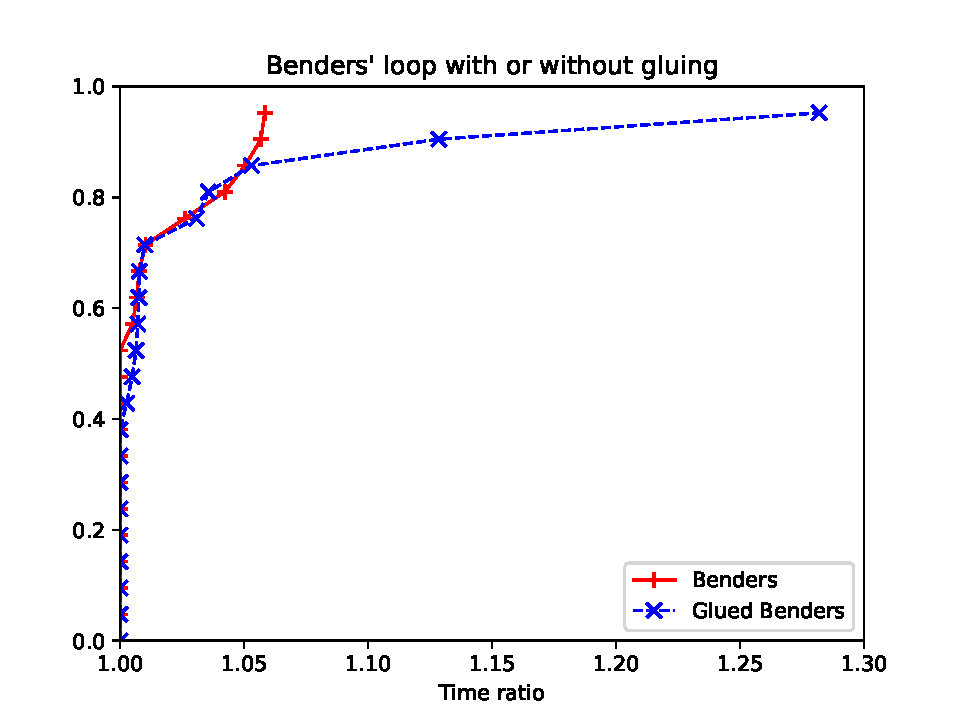
\includegraphics[width=0.7\linewidth]{Immagini/benders.pdf}
    \caption{Performance profile of Benders' loop methods.}
    \label{fig:benders_comp}
\end{figure}

The graph in Figure \ref{fig:benders_comp} compares the performance profiles of the various exact methods described in this section. 

Utilizing all available features, including MIPStart, candidate callback, user-cut callback and posting, yields the best performance, significantly improving the algorithm's efficiency and solution quality. 
Even when using only candidate callbacks and posting without MIPStart and user-cut callbacks, the performance remains highly effective, matching the best results, which indicates that posting is a particularly powerful technique within these methods. 

The B\&C approach with both callbacks is comparable with the Benders' loop method, this indicated that with the modern computational power even a more basic method is capable of performing comparably with the others.

\newpage

Overall, the analysis demonstrates that while Benders' decomposition and B\&C methods are both powerful, the strategic use of enhancements like callbacks, MIP start, and especially posting can significantly influence their performance, making them more efficient and adaptable to real-world scenarios.

\begin{figure}[H]
    \centering
    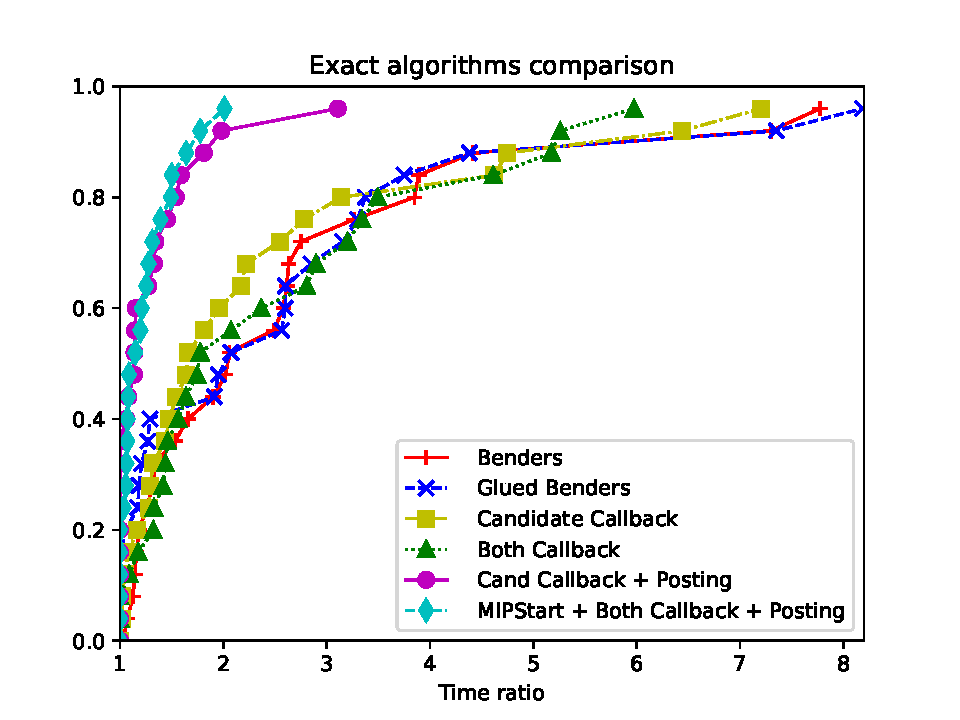
\includegraphics[width=0.7\linewidth]{Immagini/exacts.pdf}
    \caption{Performance profile of all exact methods.}
    \label{fig:exacts_comp}
\end{figure}